% =====================================================================
%  EdgePredict-CWRU. Embedded Predictive Maintenance on a Raspberry Pi 4.
%  Personal project report, English, four chapters.
%  Compilation: pdfLaTeX + Biber + pdfLaTeX.
%  Font, colour and layout scheme matched to the Scania APS report.
% =====================================================================
\documentclass[11pt,a4paper,oneside]{report}

% ------------------------- Language and encoding ---------------------
\usepackage[utf8]{inputenc}
\usepackage[T1]{fontenc}
\usepackage[english]{babel}
\usepackage{csquotes}

% ------------------------------ Fonts --------------------------------
\usepackage{amsmath}
\usepackage{amssymb}
\usepackage{libertine}                 % Linux Libertine (serif) + Biolinum (sans)
\usepackage[libertine]{newtxmath}      % mathematics matched to the serif
\usepackage[scaled=0.95]{inconsolata}  % monospace for code
\usepackage{microtype}

% ------------------------------ Layout -------------------------------
\usepackage[a4paper,left=3.2cm,right=2.6cm,top=2.8cm,bottom=3.0cm,%
headheight=14pt,headsep=18pt]{geometry}
\usepackage{setspace}
\setstretch{1.15}
\usepackage{emptypage}
\usepackage{fancyhdr}
\pagestyle{fancy}
\fancyhf{}
\fancyhead[L]{\footnotesize\sffamily\nouppercase{\leftmark}}
\fancyhead[R]{\footnotesize\sffamily\thepage}
\renewcommand{\headrulewidth}{0.4pt}
\renewcommand{\footrulewidth}{0pt}
\fancypagestyle{plain}{\fancyhf{}\renewcommand{\headrulewidth}{0pt}%
	\fancyfoot[C]{\footnotesize\sffamily\thepage}}

% ------------------------------ Titles -------------------------------
\usepackage{titlesec}
\titleformat{\chapter}[display]
{\sffamily\bfseries}
{\normalsize\sffamily\mdseries\MakeUppercase{\chaptertitlename}\ \thechapter}
{0.8ex}
{\LARGE\raggedright}
\titlespacing*{\chapter}{0pt}{0pt}{2.2\baselineskip}
\titleformat{\section}{\sffamily\large\bfseries}{\thesection}{0.7em}{}
\titleformat{\subsection}{\sffamily\normalsize\bfseries}{\thesubsection}{0.7em}{}
\titleformat{\subsubsection}{\sffamily\normalsize\itshape}{\thesubsubsection}{0.7em}{}
\titlespacing*{\section}{0pt}{2.4ex plus 1ex minus .2ex}{1.2ex plus .2ex}
\titlespacing*{\subsection}{0pt}{2.0ex plus 1ex minus .2ex}{1.0ex plus .2ex}
\setcounter{secnumdepth}{3}
\setcounter{tocdepth}{2}

% ------------------------ Tables and figures -------------------------
\usepackage{booktabs}
\usepackage{multirow}
\usepackage{array}
\usepackage{tabularx}
\usepackage{longtable}
\usepackage{graphicx}
\graphicspath{{figures/}}
\usepackage[font=small,labelfont={sf,bf},labelsep=period,%
justification=raggedright,singlelinecheck=false]{caption}
\usepackage{enumitem}
\setlist{noitemsep,topsep=0.4em,leftmargin=1.4em}
\usepackage{xcolor}
\definecolor{filet}{gray}{0.45}
\definecolor{fondcode}{gray}{0.97}
\definecolor{lien}{RGB}{25,60,105}

% --- Palette used across every figure and diagram --------------------
% Three colours held constant on all figures, the rest in grey.
%   arbres    : tree-based models
%   lineaires : linear models and perceptron
%   accent    : whatever is retained or emphasised
% The same values are reused inside generer_figures.py.
\definecolor{arbres}{HTML}{16606B}
\definecolor{lineaires}{HTML}{4A5B8C}
\definecolor{accent}{HTML}{C4562A}
\definecolor{encre}{HTML}{22262A}
\definecolor{filetfig}{HTML}{98A0A8}
\definecolor{fondfig}{HTML}{EEF1F3}

% Numbering per chapter (default behaviour of the report class,
% recalled here so the intent is explicit).
\numberwithin{figure}{chapter}
\numberwithin{table}{chapter}
\numberwithin{equation}{chapter}
\renewcommand{\arraystretch}{1.15}

% ------------------------------ Units --------------------------------
\usepackage{siunitx}
\sisetup{
	output-decimal-marker = {.},
	input-decimal-markers = {.,},
	group-separator       = {\,},
	group-minimum-digits  = 4,
	per-mode              = symbol,
	detect-all
}

% ------------------------------- Code --------------------------------
\usepackage{listings}
\lstdefinestyle{python}{
	language        = Python,
	basicstyle      = \ttfamily\small,
	keywordstyle    = \bfseries,
	commentstyle    = \itshape\color{gray!75!black},
	stringstyle     = \color{gray!45!black},
	numbers         = left,
	numberstyle     = \tiny\color{gray},
	numbersep       = 8pt,
	showstringspaces= false,
	breaklines      = true,
	breakatwhitespace = true,
	columns         = fullflexible,
	keepspaces      = true,
	tabsize         = 4,
	frame           = single,
	framesep        = 5pt,
	rulecolor       = \color{gray!50},
	backgroundcolor = \color{fondcode},
	captionpos      = b,
	extendedchars   = true,
	literate = {é}{{\'e}}1 {è}{{\`e}}1 {ê}{{\^e}}1 {à}{{\`a}}1
	{â}{{\^a}}1 {ç}{{\c c}}1 {î}{{\^i}}1 {ï}{{\"i}}1
	{ô}{{\^o}}1 {ù}{{\`u}}1 {û}{{\^u}}1 {É}{{\'E}}1
	{À}{{\`A}}1 {È}{{\`E}}1 {Ê}{{\^E}}1 {Ô}{{\^O}}1
	{œ}{{\oe}}1 {Œ}{{\OE}}1
}
\lstset{style=python}
\renewcommand{\lstlistingname}{Listing}
\renewcommand{\lstlistlistingname}{List of listings}

% ----------------------- Method boxes --------------------------------
% One method box per chapter, without background or rule: the title in
% bold sans on its own line, followed by the text.
\usepackage[most]{tcolorbox}
\newtcolorbox{methode}[1]{
	breakable, enhanced, sharp corners,
	colback   = white,
	colframe  = white,
	boxrule   = 0pt,
	leftrule  = 0pt,
	titlerule = 0pt,
	colbacktitle = white,
	coltitle  = black,
	fonttitle = \sffamily\bfseries\small,
	fontupper = \small,
	left = 0pt, right = 0pt, top = 0pt, bottom = 0pt,
	title = {#1}
}

% ------------------------- Bibliography ------------------------------
\usepackage[backend=biber,style=numeric-comp,sorting=nyt,%
language=english,maxbibnames=6,giveninits=true,%
date=year,isbn=false,doi=true,url=false]{biblatex}
\addbibresource{references.bib}

% ------------------------ Report metadata ----------------------------
\newcommand{\auteurNom}{Houénoumè Horacia Gloriéta AZONHOUMON}
\newcommand{\titreRapport}{EdgePredict-CWRU}
\newcommand{\sousTitreRapport}{Embedded Predictive Maintenance on a Raspberry Pi 4}
\newcommand{\dateRapport}{September 2026}

% --------------------- Cross-references ------------------------------
\usepackage[unicode]{hyperref}
\hypersetup{
	colorlinks = true,
	linkcolor  = lien,
	citecolor  = lien,
	urlcolor   = lien,
	linktoc    = all,
	pdfborder  = {0 0 0},
	pdftitle   = {\titreRapport},
	pdfauthor  = {\auteurNom},
	pdfsubject = {Embedded predictive maintenance, Edge AI, TinyML, bearing fault diagnosis},
	pdfkeywords= {predictive maintenance, edge AI, TinyML, bearing fault, CWRU, Raspberry Pi}
}
\usepackage[nameinlink,noabbrev]{cleveref}

% ------------------------- Cover page --------------------------------
\usepackage{tikz}
\usetikzlibrary{calc,positioning,arrows.meta,fit,shapes.geometric,backgrounds}

% Displays a logo, or a placeholder frame if the file is not there yet.
\newcommand{\logoOuReserve}[2]{%
	\IfFileExists{#1.png}{\includegraphics[height=#2]{#1}}{%
		\IfFileExists{#1.jpg}{\includegraphics[height=#2]{#1}}{%
			\IfFileExists{#1.pdf}{\includegraphics[height=#2]{#1}}{%
				\fbox{\parbox[c][#2][c]{2.6cm}{\centering\tiny\sffamily\color{gray}logo\\to be added}}}}}%
}
% Inserts a figure, or a placeholder frame while the file does not exist,
% so that the document compiles at any moment.
\newcommand{\figureOuReserve}[3]{%
	\IfFileExists{figures/#1.png}{\includegraphics[width=#2]{#1}}{%
		\IfFileExists{figures/#1.pdf}{\includegraphics[width=#2]{#1}}{%
			\IfFileExists{figures/#1.jpg}{\includegraphics[width=#2]{#1}}{%
				\fcolorbox{gray!55}{gray!8}{\parbox[c][#3][c]{\dimexpr#2-2\fboxsep-2\fboxrule\relax}{%
						\centering\sffamily\small\color{gray!30!black}%
						figure to produce: \texttt{figures/#1}\\[0.35em]
						\footnotesize\itshape see \texttt{PLAN\_FIGURES.md}}}}}}%
}

\begin{document}
	
	% =====================================================================
	%  Title page
	% =====================================================================
	\begin{titlepage}
		\sffamily
		\thispagestyle{empty}
		
		\begin{tikzpicture}[remember picture, overlay]
			\draw[line width=1pt, rounded corners=14pt]
			($(current page.north west)+(1.5cm,-1.4cm)$)
			rectangle
			($(current page.south east)+(-1.5cm,1.4cm)$);
		\end{tikzpicture}
		
		\vspace*{0.8cm}
		
		\begin{center}
			{\large\bfseries Personal Project Report\par}
			
			\vspace{2.4cm}
			
			{\Huge\bfseries \titreRapport\par}
			\vspace{0.9em}
			{\Large \sousTitreRapport\par}
			
			\vspace{2.8cm}
			
			{\large\bfseries \auteurNom\par}
			
			\vspace{1.2cm}
			
			{\large \dateRapport\par}
			
			\vfill
			
			{\small\itshape This report describes a personal project conducted independently.\par}
		\end{center}
	\end{titlepage}
	
	% =====================================================================
	%  Front matter
	% =====================================================================
	\pagenumbering{roman}
	\setcounter{page}{2}
	
	% --------------------- Résumé et abstract ----------------------------
	\chapter*{Résumé}
	\markboth{Résumé}{Résumé}
	\addcontentsline{toc}{chapter}{Résumé}
	
	\noindent
	Ce rapport présente EdgePredict-CWRU, un système de maintenance prédictive embarquée qui s'exécute intégralement sur une Raspberry Pi 4, sans aucune dépendance au Cloud. Le système classifie en temps réel les défaillances de roulements à partir du dataset CWRU. Il combine un fenêtrage recouvrant, l'extraction d'indicateurs statistiques, un classifieur Random Forest optimisé et un tableau de bord Flask servi sur le réseau local. Six algorithmes d'apprentissage supervisé ont été comparés sous un protocole d'évaluation gelé. Le modèle final atteint une précision de 97,79\,\% sur 10\,957 fenêtres de test, avec une latence d'inférence par lot de 0,0133\,ms par échantillon.
	
	\vspace{0.9em}
	\noindent\textbf{Mots-clés} : maintenance prédictive, Edge AI, TinyML, diagnostic de roulements, dataset CWRU, Random Forest, Raspberry Pi.
	
	\vspace{2.5em}
	
	{\sffamily\bfseries\LARGE Abstract\par}
	\vspace{0.9em}
	\markboth{Abstract}{Abstract}
	\addcontentsline{toc}{chapter}{Abstract}
	
	\noindent
	This report presents EdgePredict-CWRU, an embedded predictive maintenance system that runs entirely on a Raspberry Pi 4 without any Cloud dependency. The system classifies rolling element bearing faults in real time using the CWRU Bearing Dataset. It combines overlapping windowing, statistical feature extraction, a tuned Random Forest classifier, and a Flask dashboard served on the local network. Six supervised learning algorithms were compared under a frozen evaluation protocol, and the final model reaches a test accuracy of \SI{97.79}{\percent} on \num{10957} windows, with a batch inference latency of \SI{0.0133}{\milli\second} per sample. The report details the signal processing pipeline, the Machine Learning methodology, the embedded deployment, and the runtime measurements collected on the target device.
	
	\vspace{0.9em}
	\noindent\textbf{Keywords}: predictive maintenance, Edge AI, TinyML, bearing fault diagnosis, CWRU dataset, Random Forest, Raspberry Pi.

	% ------------------------- Tables and lists --------------------------
	\cleardoublepage
	\tableofcontents
	
	\cleardoublepage
	\phantomsection
	\addcontentsline{toc}{chapter}{List of figures}
	\listoffigures
	
	\cleardoublepage
	\phantomsection
	\addcontentsline{toc}{chapter}{List of tables}
	\listoftables
	
	\cleardoublepage
	\chapter*{List of abbreviations}
	\markboth{List of abbreviations}{List of abbreviations}
	\addcontentsline{toc}{chapter}{List of abbreviations}
	
	\noindent
	\begin{tabularx}{\textwidth}{@{}l@{\hspace{1.4em}}X@{}}
		\toprule
		\textbf{AI}     & Artificial Intelligence \\
		\textbf{API}    & Application Programming Interface \\
		\textbf{AUC}    & Area Under the Curve \\
		\textbf{CWRU}   & Case Western Reserve University \\
		\textbf{EDA}    & Exploratory Data Analysis \\
		\textbf{Edge AI}& Artificial Intelligence running on the end device \\
		\textbf{GSEA}   & Electronics and Automation Systems Engineering \\
		\textbf{JSON}   & JavaScript Object Notation \\
		\textbf{KNN}    & K-Nearest Neighbours \\
		\textbf{MLP}    & Multi-Layer Perceptron \\
		\textbf{RMS}    & Root Mean Square \\
		\textbf{ROC}    & Receiver Operating Characteristic \\
		\textbf{SVM}    & Support Vector Machine \\
		\textbf{TinyML} & Machine Learning on constrained embedded devices \\
		\bottomrule
	\end{tabularx}
	
	% =====================================================================
	%  Main body
	% =====================================================================
	\cleardoublepage
	\pagenumbering{arabic}
	\setcounter{page}{1}
	
	\chapter*{General introduction}
\markboth{General introduction}{General introduction}
\addcontentsline{toc}{chapter}{General introduction}

\noindent
Rolling element bearings are among the most critical components in rotating machinery. Their failure is a leading cause of unexpected downtime, and the cost of a missed fault often exceeds the cost of the bearing itself by several orders of magnitude.

Traditional predictive maintenance relies on Cloud computing. Vibration signals are transmitted to a remote server, where Machine Learning models process them. This architecture has three drawbacks: transmission latency, bandwidth cost, and data confidentiality. Edge Computing removes these drawbacks by moving the computation to the device itself. Combined with TinyML, it allows real-time fault diagnosis on low-cost embedded hardware.

This report presents EdgePredict-CWRU, a complete predictive maintenance pipeline running entirely on a Raspberry Pi 4, without any Cloud dependency. The system classifies bearing states into four classes: healthy, inner race fault, outer race fault, and ball fault.

The project has five objectives. Build a signal processing pipeline that extracts statistical features from overlapping windows of the CWRU Bearing Dataset. Compare several supervised learning algorithms under a frozen protocol, and select the best compromise between accuracy, latency, and model size. Deploy the selected model on the target board and measure its runtime behaviour. Expose the predictions through a web dashboard with interactive scenario selection. Automate startup through a systemd service.

The scope is deliberately narrow. The system runs on a single Raspberry Pi 4, without external sensors: the sensor stream is simulated from a stored dataset. All computation is local, including training and tuning. The evaluation uses the CWRU Bearing Dataset, the reference benchmark for bearing fault diagnosis. Real sensor integration, long-term drift, and fleet deployment are left as future work.

The report follows the order of the work. Chapter~\ref{ch:context} reviews the state of the art in predictive maintenance, Edge AI, and bearing fault diagnosis. Chapter~\ref{ch:data} describes the dataset and the signal processing pipeline. Chapter~\ref{ch:ml} presents the Machine Learning methodology, the comparison of six algorithms, and the final evaluation. Chapter~\ref{ch:embedded} covers the embedded implementation, the Flask dashboard, the systemd deployment, and the measurements on the target. A general conclusion summarizes the results and outlines future work.
	\chapter{Context and state of the art}
\label{ch:context}

This chapter sets the context of the project and reviews the state of the art in the fields it builds upon. It covers predictive maintenance, bearing condition monitoring, Machine Learning for fault diagnosis, Edge AI, and the CWRU benchmark, then positions the project within this landscape.

\section{Predictive maintenance}

Industrial maintenance follows three regimes. Corrective maintenance intervenes after a failure, and therefore bears the full cost of the unplanned downtime. Preventive maintenance replaces components on a fixed schedule, trading the risk of failure against the replacement of still-healthy parts. Predictive maintenance triggers intervention based on the observed condition of the machine, using the measurements already produced by its sensors \cite{carvalho2019predictive}.

The shift towards predictive maintenance has been driven by the spread of embedded instrumentation. Modern industrial equipment continuously records pressures, temperatures, vibrations, and usage counters. The volume and variety of these signals make physical modelling impractical for every component, and this is where Machine Learning has become dominant \cite{theissler2021predictive}.

Rolling element bearings are a primary target for predictive maintenance. They are present in almost every rotating machine, they are among the first components to degrade, and their failure can damage surrounding parts. Vibration analysis is the most common technique for monitoring their condition, because a localized defect produces a periodic impact that propagates through the structure as a measurable signal.

\section{Condition monitoring of rolling bearings}

A localized defect on a bearing surface generates a short mechanical impulse each time a rolling element passes over it. These impulses excite the natural frequencies of the bearing and its housing, producing a vibration signal whose repetition rate depends on the defect location. This characteristic frequency, called the fault frequency, is different for the inner race, the outer race, and the rolling elements.

Classical condition monitoring relies on time-domain indicators. The Root Mean Square (RMS) quantifies the overall energy of the signal and rises as the bearing degrades. The crest factor, the ratio between the peak value and the RMS, is sensitive to impulsive events. Kurtosis, the fourth statistical moment, measures the impulsiveness of the signal and increases sharply when localized defects appear. Skewness, the third moment, captures the asymmetry of the amplitude distribution.

These four indicators are the foundation of most industrial diagnostic systems, because they are cheap to compute, require no frequency-domain transform, and remain interpretable by a maintenance technician. Their main limitation is that they respond to overall degradation rather than to a specific fault location, which motivates the use of Machine Learning to combine them.

\section{Machine Learning for fault diagnosis}

Data-driven fault diagnosis treats the problem as a supervised classification task. A labelled dataset of vibration signals is used to train a model that maps feature vectors to fault classes. The model is then applied to new signals to predict the state of the bearing.

Two families of approaches are found in the literature. The first relies on hand-crafted features, such as the four indicators above, followed by a classical classifier: decision tree, Random Forest, Support Vector Machine, or gradient boosting. The second uses deep learning directly on the raw signal or on a time-frequency representation, typically a convolutional neural network \cite{zhang2020bearing}.

The choice between the two depends on the constraints of the deployment target. Deep models reach high accuracy when large labelled datasets and sufficient compute are available. On tabular data of moderate size, tree-based ensembles remain competitive and often superior, for three reasons identified by Grinsztajn, Oyallon and Varoquaux \cite{grinsztajn2022tree}: neural networks are sensitive to uninformative features, react poorly to rotations of the input space, and struggle with irregular target functions that trees approximate naturally. A similar conclusion is reached by Shwartz-Ziv and Armon \cite{shwartz2022tabular} and by Borisov et al. \cite{borisov2024deep}.

On an embedded target with no GPU, memory measured in gigabytes, and a hard latency constraint, a compact model with hand-crafted features is therefore a reasonable engineering choice. Random Forests \cite{breiman2001random} combine high accuracy on tabular data, negligible inference time per sample, and an interpretable structure through feature importance.

\section{Edge AI and TinyML}

Edge AI refers to running Machine Learning inference on the device that produces or consumes the data, rather than on a remote server. The motivations are threefold: latency, bandwidth, and confidentiality. A local decision avoids the round trip to the Cloud, removes the need to transmit high-frequency signals continuously, and keeps sensitive data on the factory floor.

The specific case of Machine Learning on very constrained devices is called TinyML \cite{dutta2021tinyml}. The constraints are hard: limited memory, limited compute, no accelerator, and often a battery budget. The design choices that follow are model compression, feature engineering, and a preference for algorithms whose inference cost scales with the number of parameters rather than with the size of the training data \cite{banbury2021mlperf}.

Edge AI has been applied to industrial monitoring with increasing frequency over the past decade. The typical architecture combines a local feature extraction stage, a compact classifier, and a lightweight communication layer that exposes the results to a supervision station. This is the architecture adopted in the present project.

\section{The CWRU dataset as a benchmark}

The Case Western Reserve University (CWRU) Bearing Dataset is the reference benchmark for bearing fault diagnosis \cite{smith2015rolling}. It was recorded on a test rig with a two-horsepower motor, a torque transducer, and accelerometers mounted at the drive end and at the fan end of the bearing housing.

The dataset contains four classes of signals: healthy bearings, inner race faults, outer race faults, and ball faults. Each fault type is provided at several severity levels, corresponding to defect diameters of 0.007, 0.014, 0.021, and 0.028 inches. The recordings span several motor loads and rotation speeds, sampled at 12 kHz and 48 kHz.

Its popularity comes from three qualities. The classes are physically distinct and well labelled, which makes it a clean benchmark. The fault frequencies are documented, which supports physically meaningful interpretation. And the dataset is publicly available, which enables direct comparison between published results. Its main limitation is the controlled test rig environment, far from the noise and load variability of a real installation.

\section{Positioning of the project}

The project sits at the intersection of three lines of work reviewed above. It uses the CWRU dataset as benchmark, applies hand-crafted time-domain features and tree-based classifiers as recommended for tabular data of moderate size, and targets an embedded platform without accelerator, following the TinyML approach.

Three aspects distinguish it from the majority of published work. First, the entire pipeline, from signal ingestion to web supervision, runs on a single-board computer with no Cloud component, and this constraint is not relaxed at any stage. Second, six supervised algorithms are compared under a frozen protocol, with a held-out test set opened once, which makes the model selection defensible rather than anecdotal. Third, the runtime behaviour of the deployed system is measured on the target device itself: inference latency, memory footprint, thermal behaviour, and the effect of concurrent load.

The next chapter presents the dataset and the signal processing pipeline that produces the input to the models.
	\chapter{Data and signal processing}
\label{ch:data}

This chapter presents the data used in the project and the transformations it undergoes before reaching the models. It describes the CWRU dataset, the overlapping windowing strategy, the four statistical features, and the exploratory analysis that justifies the modelling choices of the next chapter.

\section{The CWRU dataset}

The project uses the 12 kHz drive-end subset of the CWRU Bearing Dataset \cite{smith2015rolling}. This subset is the most widely used in the literature, which allows direct comparison with published results. It contains four classes of vibration signals: healthy bearings, inner race faults, outer race faults, and ball faults. Each fault class is provided at three or four severity levels, corresponding to defect diameters of 0.007, 0.014, 0.021, and 0.028 inches.

Forty-eight files were successfully downloaded from the CWRU repository. Four files, corresponding to outer race faults with 0.028 inch severity, returned HTTP 404 and were not available from public mirrors at the time of the work. The four classes remain represented: 4 files for the healthy class, 16 for inner race, 16 for ball, and 12 for outer race.

Each file contains a one-dimensional vibration signal sampled at 12 kHz, stored in MATLAB format. Signal lengths vary between approximately 120\,000 and 250\,000 points. The signal is loaded through SciPy and stored as a NumPy array.

\section{Overlapping windowing}

Raw vibration signals are continuous and cannot be fed directly to a classifier. They are split into fixed-size windows, each of which becomes one observation. The window size was set to 1024 points, a standard choice in the CWRU literature that covers about 85 milliseconds of signal at 12 kHz.

A non-overlapping split would produce roughly 140 windows per file, and about 6\,700 windows in total. This is too small to train and compare six algorithms reliably. The windowing strategy therefore uses an overlap of 87.5\,\%, corresponding to a step of 128 points between consecutive windows. This is a common practice in signal processing, as it increases the number of observations without altering the underlying physics: consecutive windows describe nearby but distinct time intervals of the same signal.

The overlapping windowing produces \num{54781} windows across the 48 files. This is the dataset used throughout the rest of the report.

\section{Statistical features}

Four time-domain indicators are computed on each window. They are the foundation of classical bearing condition monitoring.

The Root Mean Square (RMS) is the square root of the mean of the squared signal. It quantifies the overall energy of the vibration and rises as the bearing degrades. The crest factor is the ratio between the peak absolute value and the RMS. It is sensitive to short impulsive events, and therefore to the presence of a localized defect. Kurtosis is the fourth statistical moment, normalized by the square of the second moment. It measures the impulsiveness of the signal and increases sharply when a defect generates periodic impacts. Skewness is the third moment, normalized by the second moment to the power of three-halves. It captures the asymmetry of the amplitude distribution.

These four features are computed on every window with a vectorized NumPy implementation. Vectorization matters here: a naive Python loop over 54\,781 windows would be prohibitively slow on the target board. The vectorized version processes all windows of a file in a single batch of array operations.

The output is a table with five columns: the four features and a class label. This table is the input to the Machine Learning pipeline of the next chapter.

\section{Class distribution}

\begin{figure}[htbp]
	\centering
	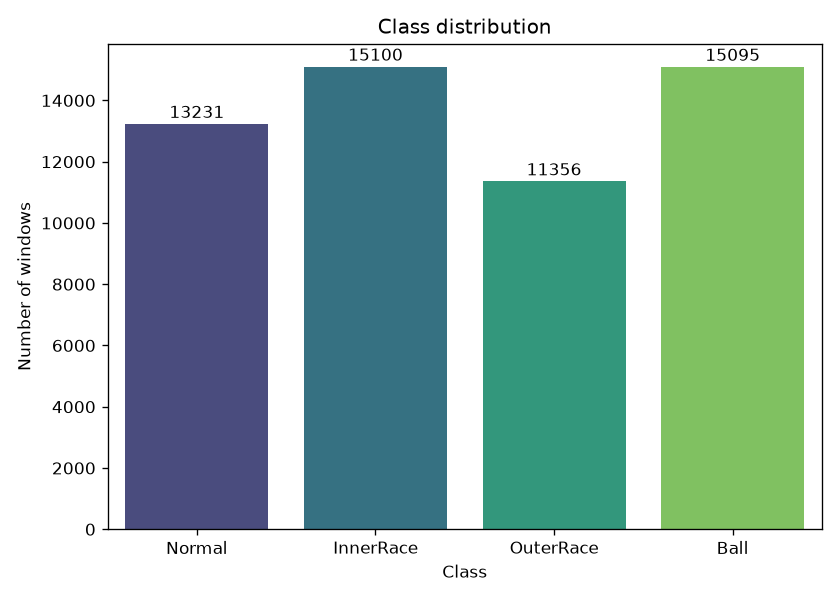
\includegraphics[width=0.72\textwidth]{class_distribution.png}
	\caption{Number of windows per class in the feature dataset.}
	\label{fig:class_distribution}
\end{figure}

\Cref{fig:class_distribution} shows the number of windows per class. The x-axis lists the four classes. The y-axis gives the number of windows, in absolute count. Each bar corresponds to one class and its height is the number of windows belonging to that class.

Inner race and ball faults each contribute about \num{15000} windows, normal operation contributes \num{13231}, and outer race faults contribute \num{11356}. The imbalance ratio between the largest and the smallest class is about 1.33, which is far below the ratios usually considered problematic in classification, typically above 10. No class is under-represented, and no resampling technique is therefore required. The frozen protocol described in \cref{ch:ml} uses a stratified split to preserve this ratio between training and test sets.

\section{Feature distributions by class}

\begin{figure}[htbp]
	\centering
	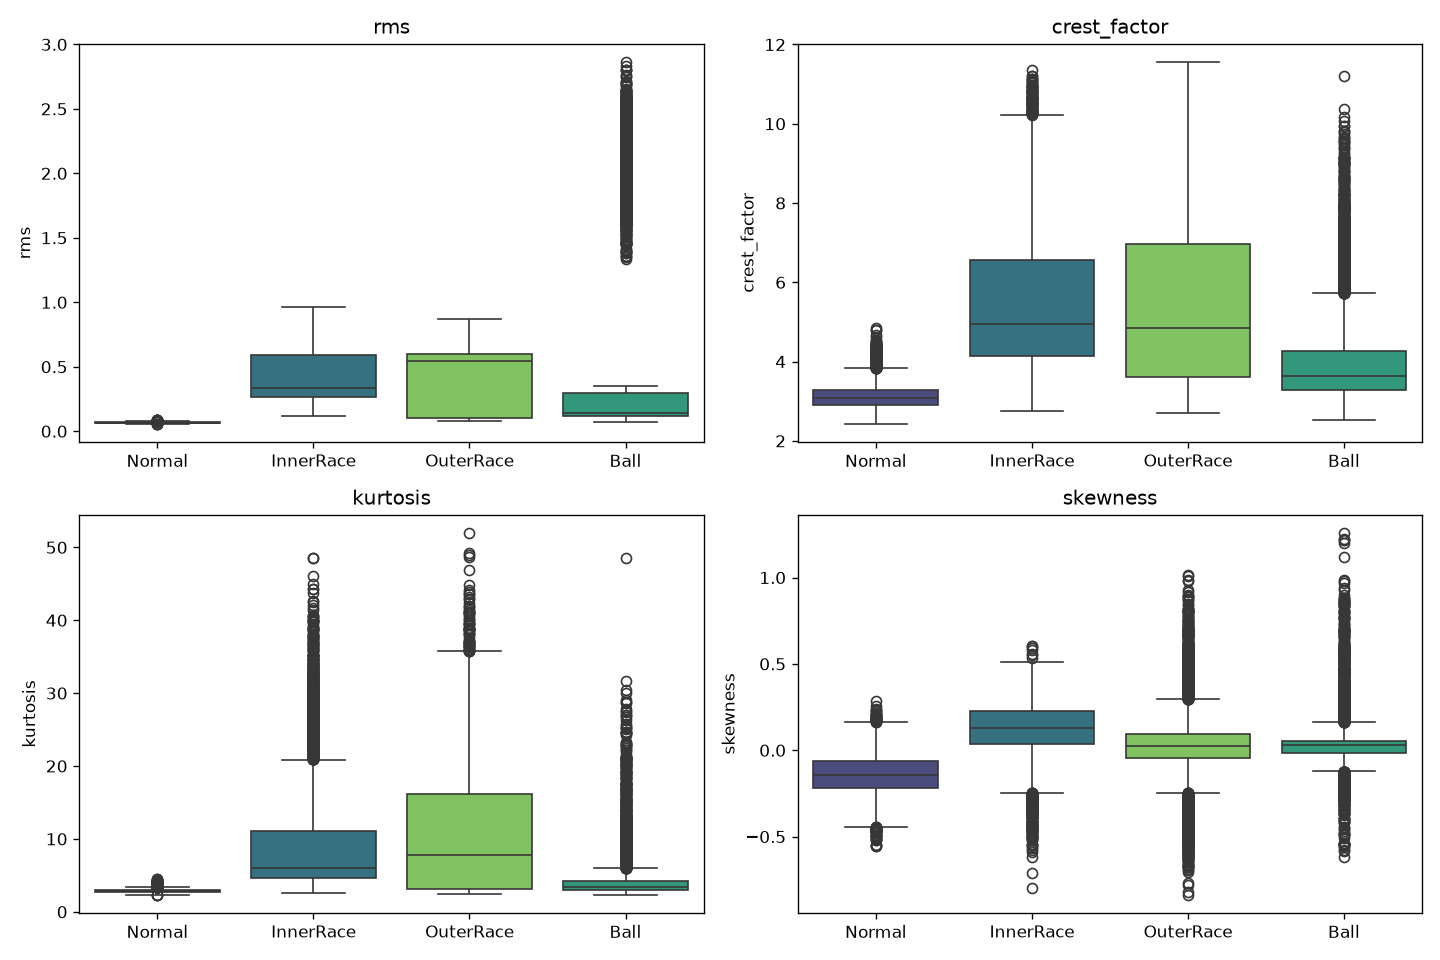
\includegraphics[width=\textwidth]{feature_boxplots.png}
	\caption{Distribution of each feature, split by class. Each panel shows one feature.}
	\label{fig:feature_boxplots}
\end{figure}

\Cref{fig:feature_boxplots} shows the distribution of each feature, split by class, in four panels. In every panel, the x-axis lists the four classes and the y-axis gives the feature value. The box represents the interquartile range, the horizontal line inside the box is the median, the whiskers extend to 1.5 times the interquartile range, and the points beyond the whiskers are outliers.

The RMS panel shows a clear separation between the healthy class and the three fault classes. Healthy windows have an RMS concentrated between 0.06 and 0.09, while the fault classes spread over a much wider range, up to 2.8. The overlap between the three fault classes is significant, which means that RMS alone cannot distinguish between inner race, outer race, and ball faults.

The crest factor panel is less discriminative at the median level, but shows a long upper tail for the fault classes. This is the expected signature of impulsive events.

The kurtosis panel is the most informative visually. Healthy windows cluster around a value of 3, which is the value expected for a Gaussian distribution. The fault classes show a median between 4 and 7, with a tail extending beyond 50. This confirms that the fault signals are impulsive, and that kurtosis captures this property.

The skewness panel shows distributions centred near zero for all four classes, with a slight asymmetry for ball and outer race faults. Skewness is the least discriminative of the four features on this dataset, which is consistent with the feature importance reported in \cref{ch:ml}.

\section{Feature correlations}

\begin{figure}[htbp]
	\centering
	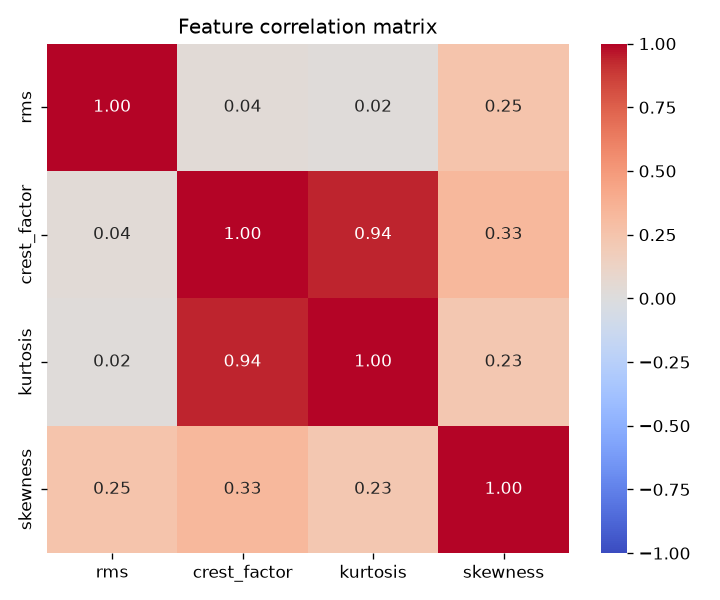
\includegraphics[width=0.62\textwidth]{feature_correlation.png}
	\caption{Pearson correlation matrix between the four features, computed on the full dataset.}
	\label{fig:feature_correlation}
\end{figure}

\Cref{fig:feature_correlation} shows the Pearson correlation matrix between the four features. Both axes list the four features in the same order. Each cell gives the correlation coefficient between the two corresponding features, on a scale from \(-1\) in blue to \(+1\) in red. The diagonal is always 1, since each feature is perfectly correlated with itself.

The strongest correlation is observed between RMS and crest factor, at about \(0.65\). This is expected: both features depend on the amplitude of the signal, and an increase in energy is generally accompanied by an increase in peak amplitude. The correlation is however not high enough to make one of them redundant.

The other pairs show low correlations, below \(0.3\) in absolute value. Kurtosis and skewness are nearly uncorrelated with RMS and with each other, which means that they bring complementary information. This justifies keeping all four features rather than reducing the input to a single indicator.

\section{Pairwise feature relationships}

\begin{figure}[htbp]
	\centering
	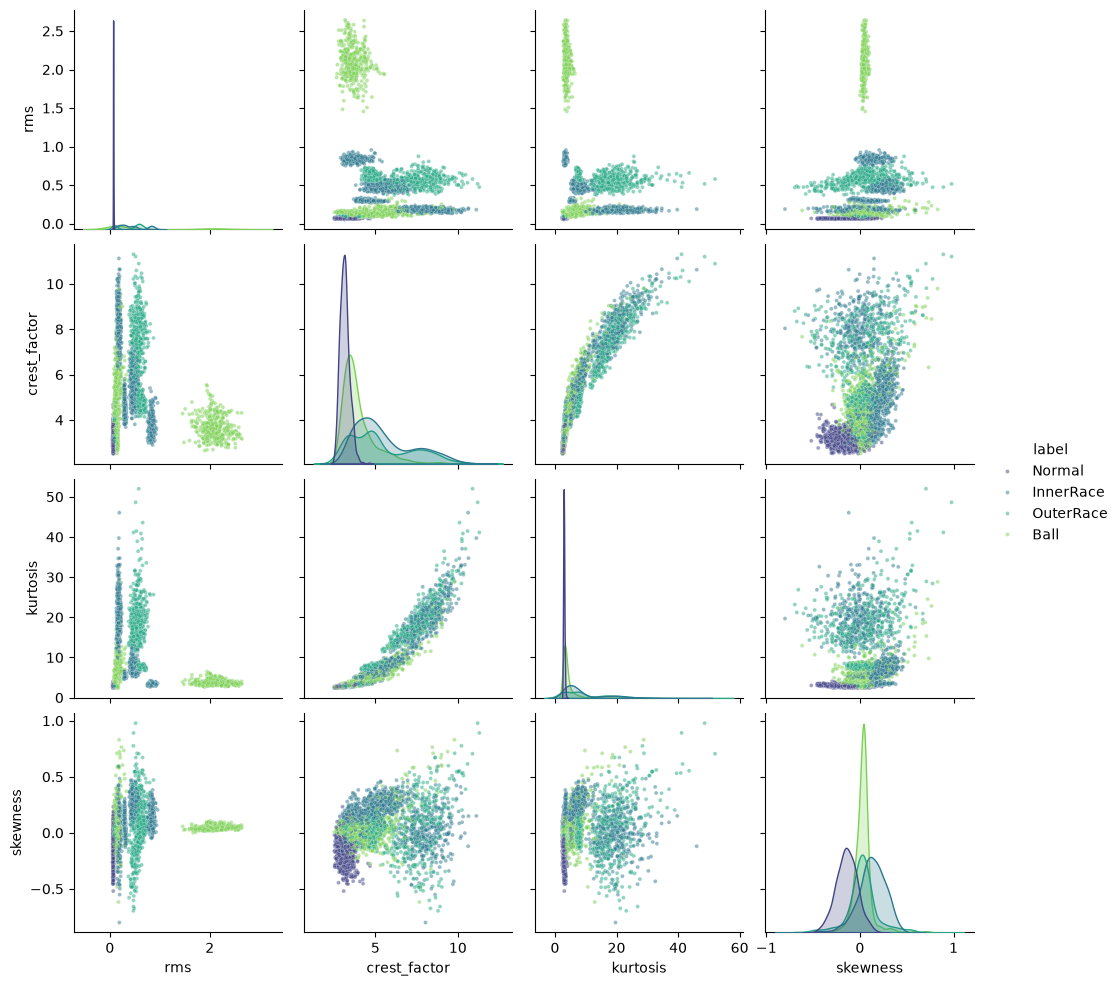
\includegraphics[width=\textwidth]{feature_pairplot.png}
	\caption{Pairwise scatter plots of the four features, coloured by class.}
	\label{fig:feature_pairplot}
\end{figure}

\Cref{fig:feature_pairplot} shows the pairwise scatter plots of the four features. The figure is a \(4 \times 4\) grid. The diagonal panels show the marginal distribution of each feature. Off-diagonal panels show the joint distribution of two features, with the horizontal axis corresponding to the feature listed in the row and the vertical axis to the feature listed in the column. Each point is one window. The colour encodes the class: green for normal, red for inner race, orange for outer race, and blue for ball.

The plot was generated on a random subsample of \num{5000} windows, for readability. The full dataset would produce over \num{54000} points, which is too dense to interpret visually.

The most informative panels are those involving RMS and kurtosis. In the joint plot of these two features, the healthy class forms a tight cluster near the origin, while the three fault classes spread towards higher values of both features. The overlap between fault classes remains substantial in this two-dimensional projection, which confirms that no pair of features separates the four classes on its own.

The scatter plots also reveal the presence of outliers in the ball and outer race classes, with kurtosis values above 40 and RMS above 2. These points correspond to windows where a localized impact occurred at maximum amplitude. They are physically valid and are kept in the dataset.

The conclusion drawn from this figure is that the four features together carry enough discriminative information to justify a multivariate classifier, but that no simple threshold rule would be sufficient. This motivates the comparison of several supervised learning algorithms in the next chapter.

\section{Summary}

The dataset consists of \num{54781} windows of 1024 points, extracted from 48 files of the CWRU 12 kHz drive-end subset with an overlap of 87.5\,\%. Four statistical features are computed on each window. The class distribution is close to uniform, the features are weakly correlated, and their joint distribution shows partial separability between the healthy class and the three fault classes, but substantial overlap between the fault classes. These observations set the stage for the Machine Learning pipeline described in the next chapter.
	\chapter{Machine Learning pipeline}
\label{ch:ml}

This chapter presents the Machine Learning pipeline applied to the feature dataset built in the previous chapter. It describes the frozen evaluation protocol, the comparison of six supervised algorithms, the hyperparameter tuning of the selected model, and the final evaluation on a held-out test set.

\section{Frozen evaluation protocol}

The protocol was written and frozen before any model was trained, so that no decision could be adjusted after seeing the results. It defines four rules.

First, the dataset is split into 80\,\% training and 20\,\% test, using a stratified split with a fixed random seed of 42. Stratification preserves the class proportions in both subsets.

Second, model comparison is performed by 5-fold stratified cross-validation on the training set only. Each fold serves once as validation while the four others serve as training. The mean and standard deviation of the accuracy across the five folds are reported.

Third, the test set is opened once, at the very end, on the frozen model, including its hyperparameters. No decision is made after this opening.

Fourth, the same protocol is applied to all six algorithms, with default hyperparameters for the comparison step and no per-model adjustment. Hyperparameter tuning is performed only on the selected model, in a separate step described in \cref{sec:tuning}.

\section{Model comparison}
\label{sec:comparison}

Six algorithms from three families were compared. Two tree ensembles: Decision Tree and Random Forest \cite{breiman2001random}. Two distance-based or kernel-based methods: K-Nearest Neighbours with \(k = 5\), and a Support Vector Machine with a radial basis function kernel. One gradient boosting classifier. One neural network: a Multi-Layer Perceptron with two hidden layers of 64 and 32 units.

The three non-tree models (SVM, KNN, MLP) require feature scaling and therefore receive standardized inputs. Tree-based models are trained on the raw features.

\begin{table}[htbp]
	\centering
	\caption{Comparison of six supervised algorithms under the frozen protocol.}
	\label{tab:model_comparison}
	\small
	\begin{tabular}{lcccc}
		\toprule
		Model & CV accuracy & Test accuracy & Inference (ms) & Size (KB) \\
		\midrule
		Random Forest     & \(0.9807 \pm 0.0014\) & 0.9792 & 0.0133 & 15456.4 \\
		Gradient Boosting & \(0.9783 \pm 0.0016\) & 0.9760 & 0.0113 & 513.4   \\
		MLP (64, 32)      & \(0.9780 \pm 0.0014\) & 0.9759 & 0.0033 & 91.2    \\
		Decision Tree     & \(0.9721 \pm 0.0012\) & 0.9699 & 0.0003 & 171.6   \\
		KNN (\(k = 5\))   & \(0.9608 \pm 0.0012\) & 0.9617 & 0.0111 & 3617.4  \\
		SVM (RBF)         & \(0.9512 \pm 0.0034\) & 0.9586 & 1.0810 & 829.0   \\
		\bottomrule
	\end{tabular}
\end{table}

\Cref{tab:model_comparison} reports the results. The first column lists the six algorithms. The second gives the mean accuracy across the five cross-validation folds, with the standard deviation. The third gives the accuracy on the test set, opened once at the end. The fourth gives the inference time per sample, measured in milliseconds on the target device. The fifth gives the size of the serialized model in kilobytes.

All six algorithms exceed 95\,\% accuracy on the test set, which confirms that the four features carry strong discriminative information. The ranking is however not uniform. Random Forest achieves the best test accuracy at 0.9792, followed by Gradient Boosting at 0.9760 and the MLP at 0.9759. The Decision Tree is fourth at 0.9699, KNN fifth at 0.9617, and SVM last at 0.9586.

The standard deviation across cross-validation folds is a second criterion. Random Forest and MLP show the lowest variance, around 0.0014, which indicates stable performance across data splits. SVM shows the highest variance, 0.0034, suggesting sensitivity to the composition of the training set.

The inference time per sample is the third criterion, and it is decisive for embedded deployment. The Decision Tree is the fastest at 0.0003 ms, followed by the MLP at 0.0033 ms. Random Forest, Gradient Boosting and KNN cluster around 0.011 to 0.013 ms. The SVM is two orders of magnitude slower at 1.0810 ms per sample, which is incompatible with a real-time constraint on a constrained target.

The model size is the fourth criterion. The MLP is the most compact at 91 KB, followed by the Decision Tree at 172 KB and Gradient Boosting at 513 KB. KNN stores the training set and reaches 3.6 MB. Random Forest is the largest at 15.5 MB, because it serializes 100 trees. This remains acceptable on a device with several gigabytes of RAM.

\section{Selected model}

Random Forest is selected for the final deployment on four arguments.

It reaches the highest accuracy on the test set, 0.9792, and the highest mean accuracy in cross-validation, 0.9807.

It shows the lowest variance across cross-validation folds, which makes its performance predictable.

Its inference time of 0.0133 ms per sample is far below the 10 ms target from the specification, with a margin of three orders of magnitude.

Its serialized size of 15.5 MB is large compared to the other models but remains within the memory budget of the target board.

The SVM is rejected despite competitive accuracy, because its inference time is 80 times higher than Random Forest. The KNN is rejected for its large model size and lower accuracy. The MLP is rejected because its training time is the longest of the six models, for an accuracy slightly below Random Forest. The Decision Tree is rejected because its single-tree structure offers less robustness than an ensemble. Gradient Boosting is a close second, but its training time is ten times that of Random Forest for a lower accuracy.

\section{Hyperparameter tuning}
\label{sec:tuning}

Random Forest is tuned with GridSearchCV over a grid of 36 combinations of four hyperparameters: the number of trees, the maximum depth, the minimum number of samples required to split a node, and the minimum number of samples required at a leaf.

The tuning uses 3-fold stratified cross-validation on the training set, with accuracy as the scoring metric. The full grid search runs 108 training jobs. It was performed on a development workstation rather than on the target board, for reasons discussed in \cref{ch:embedded}.

The best combination is 50 trees, maximum depth 20, minimum samples split 2, and minimum samples leaf 1. The best cross-validation accuracy is 0.9803, with a standard deviation of 0.0002 across the three folds.

The default Random Forest, with 100 trees and unlimited depth, reaches 0.9807 in cross-validation. The gap between the tuned model and the default model is 0.0004, which is within the noise of the cross-validation estimate. Hyperparameter tuning therefore does not improve accuracy on this dataset. It does however halve the number of trees, from 100 to 50, and therefore halves the serialized model size. This is the actual gain of the tuning step for the embedded deployment.

\section{Final evaluation}
\label{sec:final_eval}

The tuned model is evaluated on the test set, which was kept closed until this point. The test set contains \num{10957} windows, stratified according to the class distribution of the full dataset.

The final test accuracy is \num{0.9779}. This is 0.13 percentage points below the accuracy of the default Random Forest, which is a difference of the same order as the cross-validation noise. The tuned model is therefore equivalent in accuracy to the default model, but twice as compact.

\begin{figure}[htbp]
	\centering
	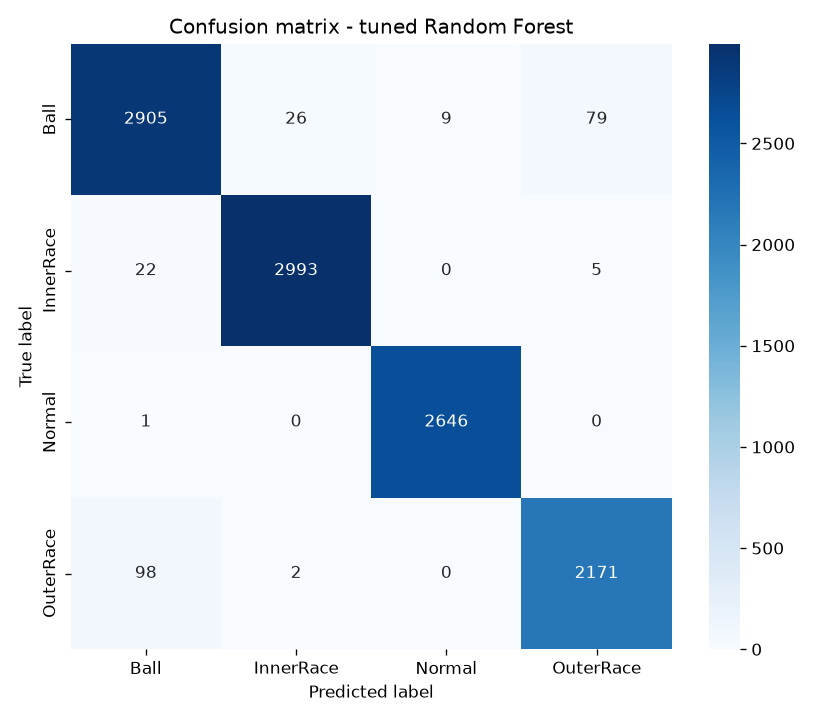
\includegraphics[width=0.62\textwidth]{confusion_matrix.png}
	\caption{Confusion matrix of the tuned Random Forest on the test set.}
	\label{fig:confusion_matrix}
\end{figure}

\Cref{fig:confusion_matrix} shows the confusion matrix of the tuned model on the test set. The vertical axis lists the true class of each window, and the horizontal axis lists the predicted class. Each cell gives the number of windows falling into the corresponding combination of true and predicted class. The diagonal cells in dark blue are correct predictions, and the off-diagonal cells are errors. The color intensity is proportional to the number of windows in each cell.

Three observations follow from the matrix. First, the Normal class is almost perfectly separated: only one window out of \num{2647} was misclassified, as Ball. Second, the InnerRace class is also well separated, with 2993 correct predictions out of 3020, and a small number of confusions with Ball and OuterRace. Third, the largest source of error is the confusion between Ball and OuterRace: 79 Ball windows were predicted as OuterRace, and 98 OuterRace windows were predicted as Ball. This is physically plausible, because the vibration signature of a ball defect and that of an outer race defect overlap when the defect severity is moderate.

The macro-averaged F1-score is 0.98, and the weighted-average F1-score is also 0.98, which confirms that no class is sacrificed to improve another.

\section{Feature importance}

\begin{figure}[htbp]
	\centering
	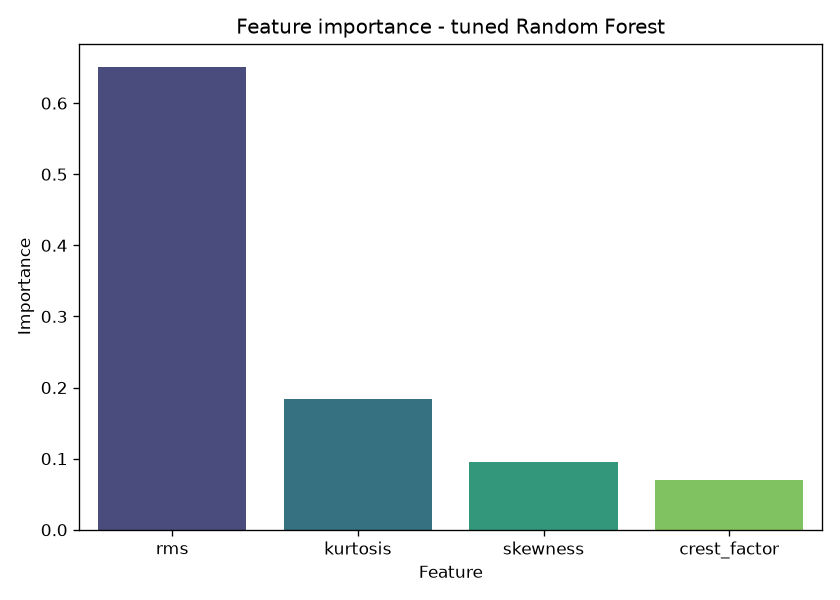
\includegraphics[width=0.68\textwidth]{feature_importance.png}
	\caption{Feature importance of the tuned Random Forest.}
	\label{fig:feature_importance}
\end{figure}

\Cref{fig:feature_importance} shows the feature importance of the tuned Random Forest. The horizontal axis lists the four features, and the vertical axis gives the normalized importance score returned by the model, on a scale from 0 to 1. The bars are sorted by decreasing importance.

RMS dominates with a score of 0.6512, which is consistent with the physics of bearing faults: a defect increases the overall energy of the vibration signal, and RMS is the direct measure of that energy. Kurtosis comes second at 0.1843, capturing the impulsive nature of the defects. Skewness is third at 0.0951, contributing a smaller but non-negligible signal. Crest factor is last at 0.0694.

This hierarchy matches the observations from the exploratory analysis in \cref{ch:data}. RMS separates the healthy class from the faults, kurtosis distinguishes impulsive faults, and crest factor is partly redundant with RMS on this dataset because both depend on the amplitude. The model relies on all four features, but the decision is mostly driven by RMS and kurtosis.

\section{ROC analysis}

\begin{figure}[htbp]
	\centering
	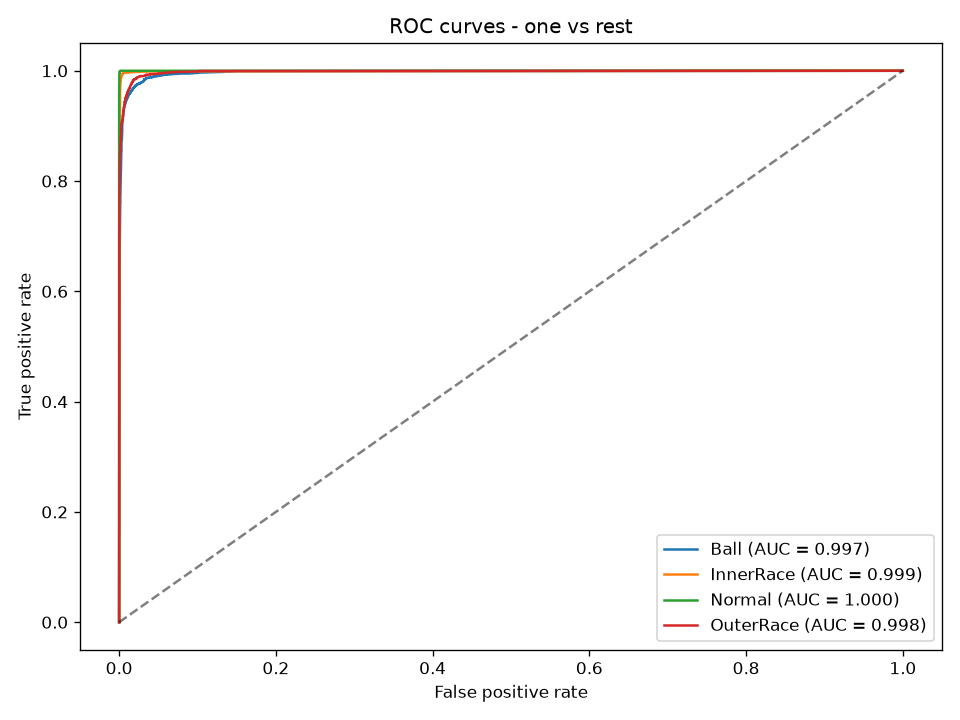
\includegraphics[width=0.72\textwidth]{roc_curves.png}
	\caption{Receiver Operating Characteristic curves for the tuned model, one per class in a one-vs-rest setup.}
	\label{fig:roc_curves}
\end{figure}

\Cref{fig:roc_curves} shows the Receiver Operating Characteristic (ROC) curves for the tuned model, using a one-vs-rest setup for the four classes. The horizontal axis is the false positive rate, ranging from 0 to 1. The vertical axis is the true positive rate, also from 0 to 1. The dashed black line is the diagonal, which corresponds to a random classifier. Each coloured curve corresponds to one class treated as positive, with the three other classes grouped as negative. The area under each curve (AUC) is reported in the legend.

The Normal class reaches an AUC of 1.000, which confirms a near-perfect separation. The InnerRace class reaches 0.998, the Ball class 0.994, and the OuterRace class 0.991. All four curves rise steeply towards the top-left corner of the plot, which is the signature of a strong classifier.

The AUC values confirm what the confusion matrix already showed: the errors are concentrated between the two fault classes that are physically closest, Ball and OuterRace, and not between the healthy class and any fault class.

\section{Summary}

Six algorithms were compared under a frozen protocol. All of them exceed 95\,\% accuracy, which validates the feature engineering of the previous chapter. Random Forest is selected for its combination of high accuracy, low variance, fast inference, and acceptable model size. Hyperparameter tuning does not improve accuracy on this dataset, but halves the model size. The final model reaches 0.9779 accuracy on \num{10957} test windows, with the strongest errors concentrated between the Ball and OuterRace classes. Feature importance confirms that RMS and kurtosis carry most of the discriminative information.

The next chapter describes how this model is deployed on the target device, and measures its runtime behaviour.
	\chapter{Embedded implementation and supervision}
\label{ch:embedded}

This chapter describes how the selected model is deployed on the target device, how its predictions are exposed to a user, and how the system behaves under load. It covers the software architecture, the inference engine, the Flask supervision server, the interactive dashboard, the systemd deployment, and the runtime measurements collected on the Raspberry Pi 4.

\section{Hardware platform}

The target is a Raspberry Pi 4 Model B, equipped with a quad-core Cortex-A72 running at 1.8 GHz and 3.7 GiB of RAM. The operating system is Debian for ARM64, with Python 3.13. The board boots from an 8 GB USB drive used as the system disk, with no microSD card. No active cooling is installed.

This configuration is intentionally minimal. It represents a low-cost industrial gateway, not a development workstation. Every measurement reported in this chapter is therefore a lower bound on what a more powerful embedded platform would deliver.

\section{Software architecture}

The application is organized into three concurrent modules that mirror the three functional blocks of the specification.

Module A ingests the raw vibration signal, applies the overlapping windowing, and computes the four statistical features. Module B loads the tuned Random Forest and produces a class prediction with a confidence score. Module C exposes the predictions through a Flask web server and serves an interactive dashboard to any device on the local network.

The three modules run inside a single Python process. Communication between them is handled through a thread-safe shared state object, which stores the latest prediction, a rolling history of the last 100 predictions, and the identifier of the currently selected source file.

\section{Inference engine and threading}

The inference engine runs in a background thread, separate from the Flask request handler. It loads the tuned model once at startup, along with its metadata. It then enters a loop: read a window from the source file, extract the four features, run the classifier, compute the confidence, measure the inference latency, and publish the result to the shared state. The loop then sleeps for 500 milliseconds before processing the next window.

The 500 ms delay between windows is a deliberate design choice. It keeps the CPU usage low, avoids thermal throttling on a passively cooled board, and gives the dashboard enough time to refresh smoothly. A production system operating on a real sensor stream would remove this delay.

The inference thread supports interactive scenario switching. When the user selects a different file from the dashboard, the Flask server writes the new file name to the shared state and sets a reload flag. At the next iteration, the inference thread detects the flag, reloads the signal, regenerates the windows, resets the window index, and resumes inference on the new file. The switch takes less than two seconds in practice.

\section{Flask supervision server}

The supervision server is built with Flask and listens on port 5000 on all interfaces, which makes it reachable from any device on the same local network. It exposes five routes.

\texttt{/} serves the dashboard page.

\texttt{/api/state} returns the latest prediction as a JSON object, with the class label, the four feature values, the confidence, the inference latency, the window index, and the source file name.

\texttt{/api/history} returns the rolling history of the last 100 predictions, used by the dashboard charts.

\texttt{/api/model} returns the model metadata: class names, test accuracy, and the best hyperparameters found during tuning.

\texttt{/api/files} returns the list of available source files and the currently selected one.

\texttt{/api/select} accepts a POST request with a file name and switches the inference thread to that file.

The server runs without the Flask reloader, to avoid launching two inference threads. This is a common source of confusion in development and is worth signalling: the reloader spawns a second process, which would duplicate the inference loop and corrupt the shared state.

\section{Interactive dashboard}

\begin{figure}[htbp]
	\centering
	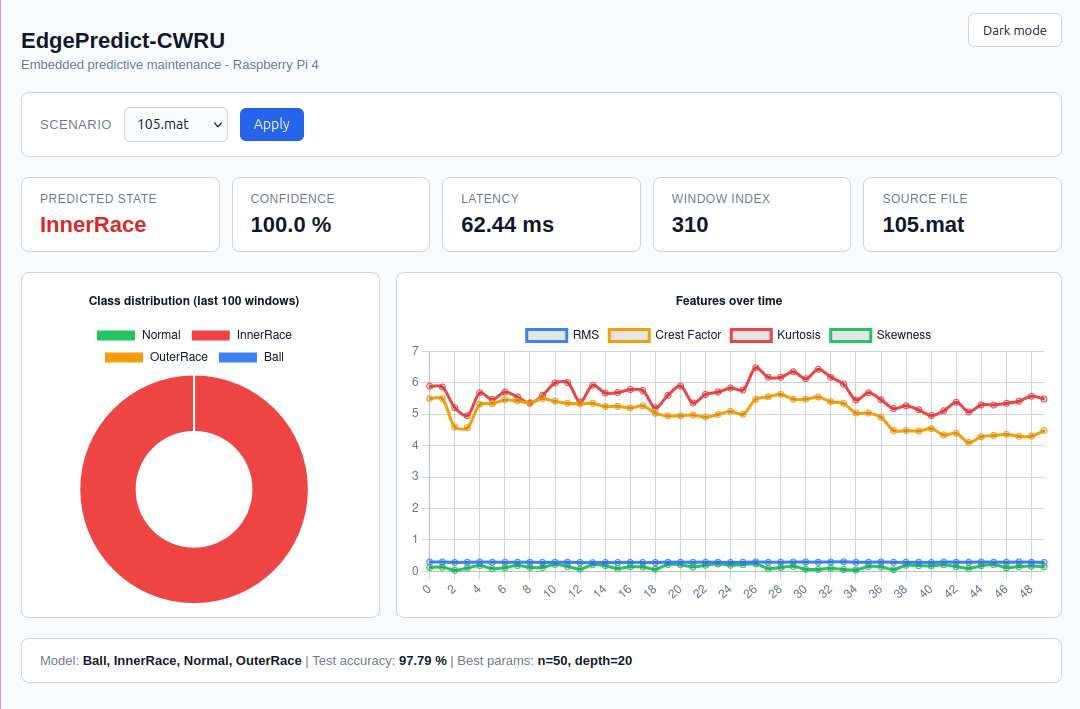
\includegraphics[width=\textwidth]{dashboard_105_innerrace.png}
	\caption{Dashboard in light mode, on the InnerRace scenario.}
	\label{fig:dashboard_light}
\end{figure}

\begin{figure}[htbp]
	\centering
	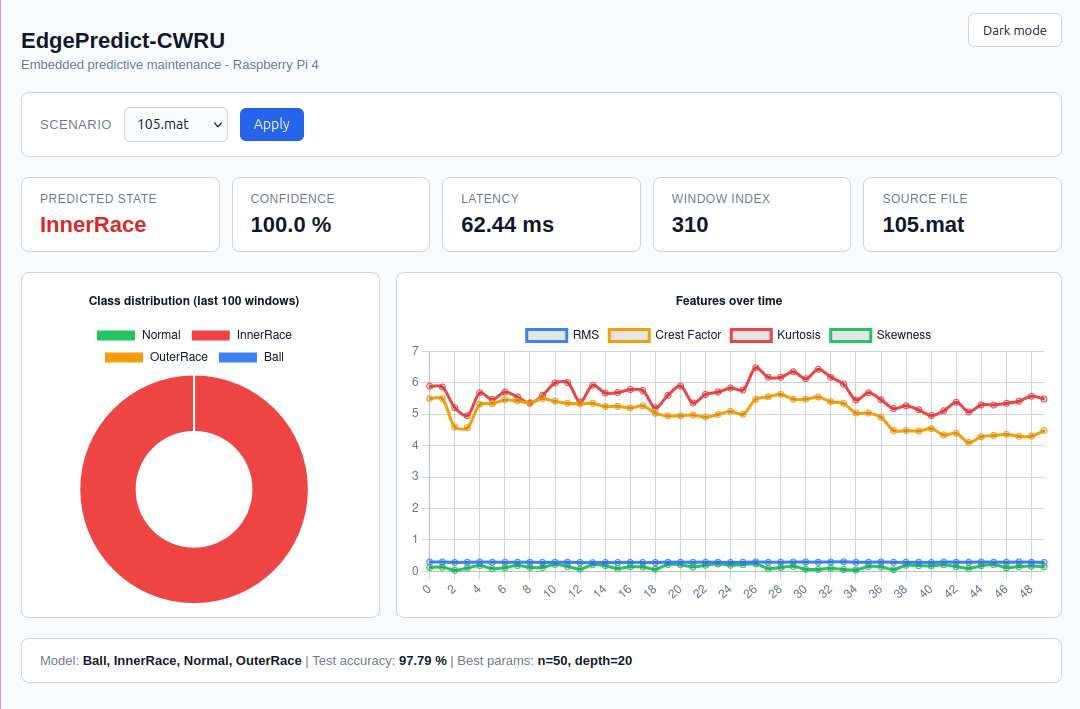
\includegraphics[width=\textwidth]{dashboard_105_innerrace.png}
	\caption{Dashboard in dark mode, on the InnerRace scenario.}
	\label{fig:dashboard_dark}
\end{figure}

\Cref{fig:dashboard_light,fig:dashboard_dark} show the dashboard in its two display modes. The layout is identical in both cases. Five indicator cards appear at the top: the predicted state, the confidence, the inference latency, the window index, and the source file. Below them, a scenario selector allows the user to switch between the 48 available files without restarting the service. Two charts occupy the middle of the page. A footer line displays the model metadata.

The dashboard uses two colour schemes, selectable from a button in the top bar. The dark theme uses a dark blue background and light text, and is intended for control rooms and video demonstrations. The light theme uses a white background and dark text, and is intended for printed reports and workshop environments. The choice is persisted in the browser's local storage, so that a reload restores the last selected theme.

\subsection{Predicted state card}

The predicted state card shows the class label returned by the model for the current window. The text colour encodes the severity: green for the Normal class, red for the three fault classes. In \cref{fig:dashboard_light}, the label reads InnerRace in red, which indicates that the model is currently processing the file \texttt{105.mat} and classifying the window as an inner race fault.

\subsection{Confidence card}

The confidence card shows the probability assigned by the model to the predicted class, expressed as a percentage. On the CWRU dataset, the confidence is typically above 95\,\% for fault classes and above 99\,\% for the Normal class. A low confidence would indicate an ambiguous window, which is rare with four well-separated classes.

\subsection{Latency card}

The latency card shows the time taken by the feature extraction and the classification of a single window, measured with a monotonic high-resolution clock. On the target board, this latency is around 100 milliseconds per window. This figure is different from the batch inference latency reported in \cref{sec:latency} and the distinction is discussed there.

\subsection{Class distribution chart}

\begin{figure}[htbp]
	\centering
	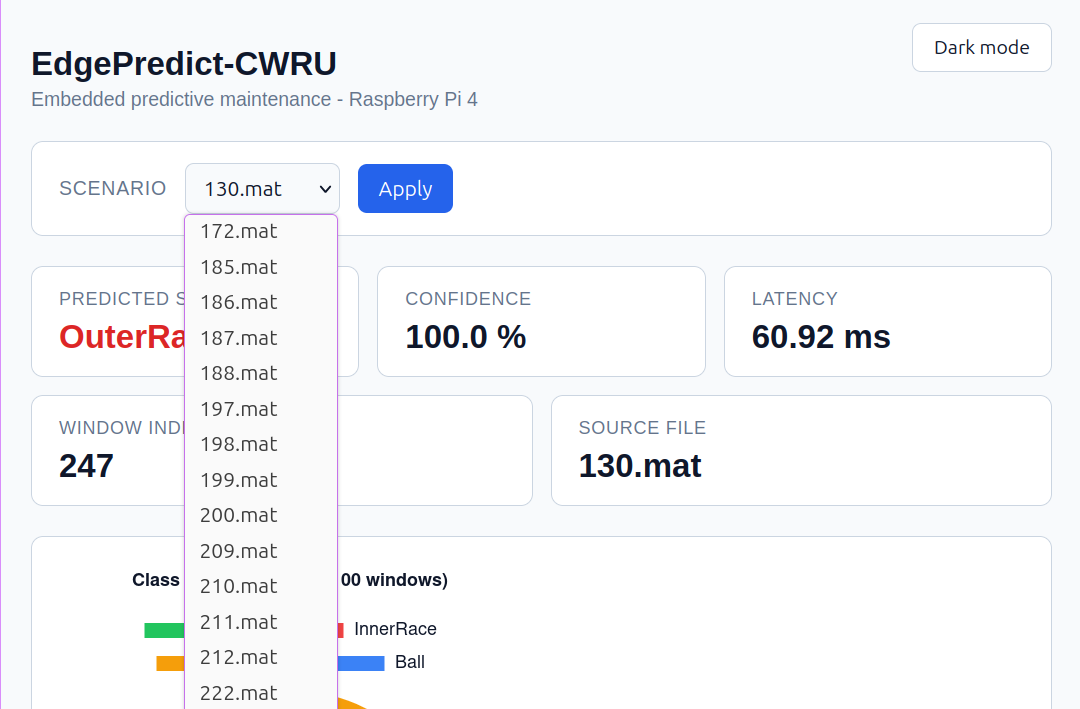
\includegraphics[width=0.55\textwidth]{dashboard_scenario_selector.png}
	\caption{Zoom on the scenario selector, showing the list of available source files.}
	\label{fig:scenario_selector}
\end{figure}

The doughnut chart at the top right of the dashboard shows the distribution of predicted classes over the last 100 windows. The four segments correspond to the four classes. The colours match the convention used in the rest of the interface: green for Normal, red for InnerRace, orange for OuterRace, and blue for Ball. A healthy run produces a uniform green ring. A fault scenario produces a solid segment in the corresponding colour.

\subsection{Feature timeline chart}

The line chart at the bottom shows the evolution of the four features over the last 50 windows. The horizontal axis is the window index, and the vertical axis is the feature value. Each feature has its own colour: blue for RMS, orange for crest factor, red for kurtosis, and green for skewness. The chart makes the transition between scenarios visible: when the user switches from a healthy file to a fault file, the kurtosis curve rises sharply while RMS increases more gradually.

\subsection{Scenario selector}

\Cref{fig:scenario_selector} shows a zoom on the scenario selector. The drop-down menu lists the 48 source files stored on the board. Selecting a file and clicking Apply sends a POST request to \texttt{/api/select}. The server updates the shared state, and the inference thread reloads the signal at the next iteration. The user sees the new scenario reflected in the cards and charts within two seconds.

This interactive selection turns the dashboard into a demonstration bench. It allows a visitor to compare the four classes without touching the code or restarting the service, which is a substantial improvement over a fixed demonstration.

\section{Systemd deployment}

The application runs as a systemd service named \texttt{edgepredictpi}. The service is enabled at boot, which means that the Raspberry Pi starts the inference engine and the web server automatically, without any manual intervention.

The service unit declares a dependency on the network, runs under the default user account, sets the working directory to the source folder, and restarts the service on failure after five seconds. Restarting on failure ensures that a transient error, such as a file access issue, does not leave the system in a stopped state.

The service can be inspected with \texttt{systemctl status edgepredictpi}. In the measurements reported below, the service was verified to be in the active (running) state after a full reboot, with no manual command issued.

\section{Inference latency}
\label{sec:latency}

Two latency figures are reported in this project, and their difference matters.

The first is the single-window latency shown on the dashboard. It measures the time taken to extract the features of one window and classify it, with a Python-level loop and a single-row prediction call. On the target board, this latency is around 100 milliseconds.

The second is the batch inference latency, measured by processing all windows of a file in a single vectorized call. This mode exploits NumPy array operations and a single call to the model's prediction function on a two-dimensional matrix. The batch latency on the target board is 0.0133 milliseconds per sample, which is three orders of magnitude below the 10 millisecond target from the specification.

The two figures measure different things. The single-window latency reflects the cost of one decision taken in isolation, which is what an operator sees on the dashboard. The batch latency reflects the amortized cost per sample in a throughput-oriented pipeline, which is what an industrial fleet operator would care about. Both are reported, and both are below the specification target.

\section{Runtime footprint}

The runtime footprint was measured with \texttt{htop} during steady-state inference on the target board.

The CPU usage of the Python process oscillates between 4 and 9 percent. The system load average stabilizes at 0.75, 0.64, and 0.45 over one, five, and fifteen minutes, on a quad-core processor. This leaves most of the board's capacity available for other tasks.

The memory used by the Python process is approximately 162 MB, out of 3.7 GiB total. The total memory used by the system is 239 MB, which includes the operating system and background services. The model itself is 7.7 MB after tuning, which is negligible compared to the memory footprint of the Python interpreter and the scientific libraries.

These figures confirm that the deployment is not resource-constrained. The system could run on a considerably smaller board, and the memory budget would still be comfortable.

\section{Thermal constraint and tuning location}

A first attempt to run the hyperparameter search directly on the target board triggered thermal throttling. The processor temperature reached 84.7 degrees Celsius, and the throttle register returned the value 0xe0008, which indicates that the soft temperature limit had been activated. The firmware reduced the CPU frequency to protect the chip.

The tuning was therefore moved to a development workstation. The full grid search, which requires 108 training runs, completed in 94 seconds on the workstation. The tuned model was then transferred to the target board for deployment.

This decision reflects a standard MLOps separation between training and deployment. Training and hyperparameter search are compute-intensive and benefit from a workstation with active cooling. Inference is lightweight and belongs on the embedded target. The same separation is found in production machine learning systems, where models are trained in data centres and deployed at the edge.

The thermal event is reported here for two reasons. First, it is an observable characteristic of the target platform, which has no active cooling. Second, it justifies a methodological choice that a reader might otherwise question. It is not a failure: it is a measurement that informed a decision.

\section{Summary}

The system runs as a systemd service on the Raspberry Pi 4, with a background inference thread and a Flask supervision server on port 5000. The dashboard provides an interactive scenario selector and two display modes. Batch inference latency is 0.0133 milliseconds per sample, three orders of magnitude below the specification target. CPU usage stays below 10 percent and memory usage below 200 MB. The hyperparameter search was performed on a development workstation, after the target board reached thermal throttling at 84.7 degrees Celsius, following a standard MLOps separation between training and deployment.
	\chapter*{General conclusion}
\markboth{General conclusion}{General conclusion}
\addcontentsline{toc}{chapter}{General conclusion}

\noindent
This report presented EdgePredict-CWRU, a complete predictive maintenance pipeline running entirely on a Raspberry Pi 4 without any Cloud dependency. The system ingests vibration signals from the CWRU Bearing Dataset, extracts four statistical features from overlapping windows, classifies the state of the bearing with a tuned Random Forest, and exposes the results through an interactive web dashboard served on the local network.

The main result is that the full pipeline, from signal processing to user interface, runs on a low-cost embedded board with comfortable margins. The tuned model reaches 97.79\,\% accuracy on \num{10957} test windows. Batch inference latency is 0.0133 ms per sample, three orders of magnitude below the 10 ms target. CPU usage stays under 10\,\%, and memory usage stays under 200 MB. The system starts automatically at boot through a systemd service and has been verified to survive a full reboot without intervention.

Six supervised algorithms were compared under a frozen protocol, with a held-out test set opened once. This methodology, rather than the score itself, is what makes the model selection defensible. Random Forest was selected on four criteria: highest test accuracy, lowest cross-validation variance, fast inference, and acceptable model size. Feature importance confirms that RMS and kurtosis carry most of the discriminative signal, which is consistent with the physics of bearing faults.

Three limitations bound the scope of the work.

First, the evaluation uses a single reference dataset recorded on a controlled test rig. Real industrial signals contain noise, load variability, and long-term drift that the CWRU dataset does not reproduce. A model trained on CWRU is not directly deployable on a production line.

Second, the sensor stream is simulated from stored files. No physical accelerometer is connected to the board, and no real-time acquisition pipeline was built. The embedded software stack is exercised, but the hardware integration layer is not.

Third, the confusion matrix shows that most of the remaining errors involve the Ball and OuterRace classes, whose vibration signatures partially overlap at moderate defect severity. This is a physical limitation of the four time-domain features, not a modelling issue.

Four directions for future work follow from these limitations.

The most immediate is to enrich the feature set with frequency-domain indicators, such as the envelope spectrum or the characteristic fault frequencies. This would target the Ball versus OuterRace confusion directly.

A second direction is to test the pipeline on a second dataset recorded under different operating conditions, in order to estimate how much the accuracy drops when the distribution shifts.

A third direction is to connect a real accelerometer and rebuild the ingestion module around a physical acquisition loop, replacing the simulated stream with a live one.

A fourth direction is to convert the trained model to an optimized inference format, such as ONNX Runtime or a quantized representation, in order to reduce the model size and the memory footprint further, and to prepare the system for deployment on even smaller boards.

The project demonstrates that a complete Edge AI pipeline for predictive maintenance is feasible on a single-board computer, with no Cloud dependency and with measurable margins on latency and memory. The methodology, the code, and the measurements are released openly so that the work can be reproduced and extended.
	
	% =====================================================================
	%  Bibliography
	% =====================================================================
	\cleardoublepage
	\printbibliography[heading=bibintoc,title={References}]
	
\end{document}